% smrdoc.tex V2.10, 13 July 2012
\documentclass[times]{smrauth}
%When you submit your paper, please use the command
%\def\baselinestretch{2}
% or \documentclass[times, doublespace]{smrauth}

% Syntax package configuration
\usepackage[rounded]{syntax}
\setlength{\grammarparsep}{4pt plus 1pt minus 1pt}

% multiple images
\usepackage{subcaption}

% Parse trees
\usepackage{forest}

\usepackage[hyphens]{url}
\usepackage[hidelinks]{hyperref}

\usepackage{rotating}
\usepackage[utf8]{inputenc}
\usepackage[T1]{fontenc}

\begin{document}

\runningheads{E.~Aivaloglou et al.}{A bulletproof grammar for spreadsheet formulas}

\title{A bulletproof grammar for spreadsheet formulas}

\author{Efthimia Aivaloglou\affil{1}\corrauth, David Hoepelman\affil{1}, Felienne Hermans\affil{1}}

\address{Software Engineering Research Group, Delft University of Technology, Mekelweg 4, 2628 CD Delft, The Netherlands}

\corraddr{Software Engineering Research Group, Delft University of Technology, Mekelweg 4, 2628 CD Delft, The Netherlands. E-mail: e.aivaloglou@tudelft.nl}

\begin{abstract}
Spreadsheets are ubiquitous in the industrial world and often perform a role similar to other computer programs, which makes them interesting research targets.
However, there does not exist a reliable grammar that is concise enough to facilitate formula parsing and analysis and to support research on spreadsheet codebases.

This paper presents a grammar for spreadsheet formulas that is compatible with the spreadsheet formula language, is compact enough to feasibly implement with a parser generator, and produces parse trees aimed at further manipulation and analysis. 
We evaluate the grammar against more than eight million unique formulas extracted from four spreadsheet datasets, successfully parsing 99.99\%.
Additionally, we utilize the grammar to analyze these datasets and measure the frequency of usage of language features in spreadsheet formulas.
Finally, we identify smelly constructs and uncommon cases in the syntax of formulas.
\end{abstract}

\keywords{spreadsheets; syntax; formula grammar}

\maketitle

\section{Introduction}
Spreadsheets are widely used in industry: Winston~\cite{Wins2001} estimates that 90\% of all analysts in industry perform calculations in
spreadsheets. Their use is diverse, ranging from inventory administration to educational applications and from scientific
modeling to financial systems. It is estimated that 90\% of desktops have Excel installed \cite{DBLP:conf/icse/BradleyM09} and that the number of spreadsheet programmers is bigger than that of software programmers \cite{DBLP:conf/vl/ScaffidiSM05}. 

Because of their widespread use, spreadsheets have been the topic of research since the nineties \cite{DBLP:journals/sigplan/BellP93}. Recent research has often focused on analyzing and visualizing spreadsheets \cite{DBLP:conf/icse/HermansPD11, Shio1999}. More recently, researchers have attempted to define \emph{spreadsheet smells}: applications of Fowler's code smells to spreadsheets \cite{DBLP:conf/icse/HermansPD12, DBLP:conf/icsm/Hermans212}, followed by approaches to refactor spreadsheets \cite{hermans2014bumblebee,badame2012refactoring}. These research works analyze the formulas within spreadsheets, and therefore often involve formula parsing. This is done either by using simple grammars which have not been evaluated (\cite{badame2012refactoring}), or through implied, undefined grammars (\cite{DBLP:conf/icse/HermansPD11,DBLP:conf/icse/HermansPD12, DBLP:conf/icsm/Hermans212, hermans2014bumblebee}). 

The above analyses are our main motivation towards a defined grammar. Having such a grammar will enable parsing spreadsheet formulas into processable parse trees which can in turn be used to analyze cell references, extract metrics, find code smells and explore the structure of spreadsheets. Essentially, a reliable and consistent grammar and its parser implementation, available to the spreadsheet research community, can support research on spreadsheet formula codebases and can enhance the understanding and usability of research results.

To make a grammar suitable for this goal, the requirements that we set for it are (1) to be compatible with the official Excel formula language, (2) to produce parse trees suited for further manipulation and analysis, and (3) to be compact enough to feasibly implement with a parser generator. The approach that we took towards developing the grammar was gradual enrichment through trial-and-error: we started from a simple grammar containing only the most common and well known formula structures and implemented it using a parser generator. Then we repeatedly tested it against formulas extracted from spreadsheet datasets, leading to further enrichments and refinements, until all common and rare cases found in the datasets were supported.
We used the three major datasets that are available in the spreadsheet research community, namely the EUSES \cite{euses}, the Enron \cite{enron} and the FUSE corpus \cite{fuse}, along with a dataset that we accumulated through web crawling, jointly containing over three hundred spreadsheets.

The contributions of this paper are (1) a concise grammar for spreadsheet formulas, (2) the evaluation of the compatibility of the grammar using four major datasets, and (3) an analysis of the common formula characteristics and of the rare grammatical cases in the datasets.

The remainder of the paper is organized as follows: In the following section we summarize the basic concepts of spreadsheets and of the formula language. In Section \ref{section:grammar} we present the spreadsheet formula grammar, its lexical and syntactical analysis rules, and details on precedence and ambiguity. Section \ref{sec:evaluation} explains how we implemented and evaluated the grammar, presents the obtained results, and analyses the formula characteristics of the datasets. In Section \ref{sec:discussion} we discuss the grammar and its limitations. Section \ref{section:relatedWork} presents related work and Section \ref{section:conclusion} concludes the paper.

\section{Background}

Spreadsheets are cell-oriented dataflow programs which are Turing complete \cite{ExcelTuringComplete}.
A single spreadsheet \emph{file} corresponds to a single (\emph{work})\emph{book}.
A workbook can contain any number of (\emph{work})\emph{sheets}.
A sheet consists of a two-dimensional grid of \emph{cells}.
The grid consists of horizontal \emph{rows} and vertical \emph{columns}.
Rows are numbered sequentially top-to-bottom starting at 1, while columns are numbered left-to-right alphabetically, i.e. base-26 using A to Z as digits, starting at `A', making column 27 `AA'.

A cell can be empty or contain a \emph{constant value}, a \emph{formula} or an \emph{array formula}.
Formulas consist of expressions which can contain constant values, arithmetic operators and \emph{function calls} such as \texttt{SUM(\ldots)} and, most importantly, \emph{references} to other cells.
Functions can be built-in or user-defined (UDFs).

\subsection{References}
References are the core component of spreadsheets.
The value of any cell can be used in a formula by concatenating its column and row number, producing a reference like \texttt{B5}.
If the value of a cell changes this new value will be propagated to all formulas that use it.

When copying a cell to another cell by default references will be adjusted by the offset, for example copying \texttt{=A1} from cell B1 to C2 will cause the copied formula to become \texttt{=B2}.
This can be prevented by prepending a \texttt{\$} to the column index, row index or both.
The formula \texttt{=\$A\$1} will remain the same on copy while \texttt{=\$A1} will still have its row number adjusted.

References can also be \emph{ranges}, which are collections of cells.
Ranges can be constructed by three operators: the range operator \texttt{:}, the union operator \texttt{,} (a comma) and the intersection operator \texttt{\char32} (a single whitespace).
The range operator creates a rectangular range with the two cells as top-left and bottom-right corners, so \texttt{=SUM(A1:B10)} will sum all cells in columns A and B with row number 1 through 10.
The range operator is also used to construct ranges of whole rows or columns, for example \texttt{3:5} is the range of the complete rows three through five.
The union operator, which is different from the mathematical union as duplicates are allowed, combines two references, so \texttt{A1,C5} will be a range of two cells, \texttt{A1} and \texttt{C5}.
Lastly the intersection operator returns only the cells which are occurring in both ranges, \texttt{=A:A 5:5} will thus be equivalent to \texttt{=A5}.

A user can also give a name to any collection of cells, thus creating a \emph{named range} which can be referenced in formulas by name.

\subsection{Sheet and External References and DDE}
\label{subsection:ExternalRefsDDE}

By default references point to cells or ranges in the same sheet as the formula, but this can be modified with a prefix. A prefix consists of an identifier, followed by an exclamation mark, followed by the actual reference.

A reference to another sheet in the same workbook is indicated using the sheetname as prefix: \texttt{=Sheetname!A1}. References to external spreadsheet files are defined by prepending the file name in between square brackets: \texttt{=[Filename]Sheetname!A1}.
A peculiar type of prefix are those that indicate multiple sheets: \texttt{=Sheet1:Sheet10!A1} means cell A1 in Sheet1 through Sheet10.
Sheet names are enclosed in single quotes if they contain special characters or spaces, e.g. \texttt{='Sheetname with space'!A1}. 

\subsection{Array Formulas and Arrays}
\label{sec:arrayformulas}
In spreadsheet programs it is possible to work with one- or two-dimensional matrices. When constructed from constant values they are called \emph{array constants}, e.g. \texttt{\{1,2;3,4\}}.
They are surrounded by curly brackets, columns are separated by commas, and rows by semicolons.
Several matrix operations are available, for example \texttt{=SUM(\{1,2,3\}*10)} will evaluate to 60.

\emph{Array Formulas} use the same syntax as normal formulas, except that the user must signal that it is an array formula, usually by pressing \emph{Ctrl} + \emph{Shift} + \emph{Enter}.
Marking a formula as an array formula will enable one- or two-dimensional ranges to be treated as arrays.
For example, if \texttt{A1},\texttt{A3},\texttt{A3} contain the values \texttt{1},\texttt{2},\texttt{3}, the array formula \texttt{\{=SUM(A1:A3*10)\}} will evaluate to \texttt{60}.

\section{Spreadsheet Formula Grammar}
\label{section:grammar}

For previous and ongoing research the authors needed a grammar for Microsoft Excel spreadsheet formulas with the following requirements:

\label{sec:designgoals}
\begin{enumerate}
	\item Compatibility with the official language
	\item Produce parse trees suited for further manipulation and analysis with minimal post-processing required
	\item Be compact enough to feasibly implement with a parser generator
\end{enumerate}

While an official grammar for Excel formulas is published \cite{ExcelOfficialGrammar}, it does not meet the above requirements for two reasons: first, it is over 30 pages long and contains hundreds of production rules and thus fails requirement 3.
Second, because of the detail of the grammar and the large number of production rules, the resulting parse trees are very complex and thus fail requirement 2.
An example is given in Figure \ref{figure:parsetrees}(a): the relatively simple formula \texttt{SUM(B2,5)} results in a 37-node tree with a depth of 18 nodes.

For these reasons the authors decided to construct a new grammar with the above requirements as design goals.

\begin{figure}
	\centering
	\begin{subfigure}[b]{0.45\textwidth}
		\centering
		\hspace{-2em}
		\scalebox{.7}{
			\begin{forest}
		[formula
			[expression
				[nospace-expression
					[function-call
						[\texttt{SUM}]
							[sum-params
								[\texttt{(}]
								[argument[argument-expression
									[ref-argument-expression
										[ref-argument-nospace-expression
											[cell-reference
												[local-cell-reference
													[A1-reference
														[A1-cell
															[A1-column
																[A1-relative-column
																	[letter[\texttt{B}]]
																]
															]
															[A1-row
																[A1-relative-row
																	[row-digit-sequence
																		[nonzero-decimal-digit[\texttt{2}]]
																	]
																]
															]
														]
													]
												]
											]
										]
									]
								]]
								[\texttt{,}]
								[argument[argument-expression
									[nospace-argument-expression
										[constant
											[numerical-constant
												[significand-part
													[whole-number-part
														[digit-sequence
															[decimal-digit[\texttt{5}]]
														]
													]
												]
											]
										]
									]
								]]
								[\texttt{)}]
							]
						]
					]
				]
			]
		]
	\end{forest}
		}
		\caption{Microsoft Excel parse tree, constructed based on reference \cite{ExcelOfficialGrammar}}
	\end{subfigure}
	~
	%\end{figure}
	%\begin{figure}
	\begin{subfigure}[b]{0.45\textwidth}
		\centering
		\vspace{1em}
		\hspace{-0.5em}
		\scalebox{.7}{
				\begin{forest}
			[Formula
				[FunctionCall
					[EXCEL-FUNCTION[{\texttt{SUM(}}]]
					[Arguments
						[Argument[Formula
							[Reference
								[ReferenceItem
									[CELL
										[\texttt{B2}]
									]
								]
							]
						]]
						[\texttt{,}]
						[Argument[Formula
							[Constant
								[NUMBER[\texttt{5}]]
							]
						]]
					]
					[{\texttt{)}}]
				]
			]
	\end{forest}
		}
		\caption{Parse tree produced using the grammar defined in this paper}
	\end{subfigure}
	\caption{Parse trees for formula \texttt{SUM(B2,5)}}
	\label{figure:parsetrees}
\end{figure}

\subsection{Grammar Class}

While the class of this grammar is not strictly LALR(1) due to the ambiguity discussed in Section \ref{sec:ambiguity}, we implemented this grammar using a LALR(1) parser generator.
The present ambiguity can be solved by defining operator precedence (section \ref{sec:operatorprecedence}) and manually resolving conflicts (Section \ref{sec:ambiguity}).
These two features are supported by most LALR(1) parser generators.

\subsection{Lexical Analysis}
Table \ref{table:tokens} contains the lexical tokens of the grammar, along with their identification patterns in the regular expression language. All tokens are case-insensitive.
Characters are defined as unicode characters x9,xA,xD and x20 and upwards.

\begin{sidewaystable}
	\vspace{2mm}
	\caption{Lexical tokens used in the grammar}
	\label{table:tokens}
	\centering
	\stepcounter{footnote}

\begin{tabular}{@{}llll@{}}
\toprule
Token Name & Description & Contents & Priority \\
\midrule
%BINOP & Binary Operator & + $\mid$ - $\mid$ / $\mid$ * $\mid$ \textasciicircum $\mid$ \textless $\mid$ \textgreater $\mid$ = $\mid$ \textless= $\mid$ \textgreater= $\mid$ \textless \textgreater & 0 & + \\
BOOL & Boolean literal & TRUE $\mid$ FALSE & 0 \\
CELL & Cell reference & \$? [A-Z]+ \$? [0-9]+ & 2 \\
DDECALL & Dynamic Data Exchange link & ' ([\textasciicircum{} '] $\mid$ '')+ ' & 0 \\
ERROR & Error literal & \begin{tabular}[c]{@{}l@{}} \#NULL! $\mid$ \#DIV/0! $\mid$ \#VALUE! \\ $\mid$ \#NAME? $\mid$ \#NUM! $\mid$ \#N/A \end{tabular} & 0 \\
ERROR-REF & Reference error literal & \#REF! & 0 \\
EXCEL-FUNCTION & Excel built-in function & (Any entry from the function list\begin{footnotesize}\textsuperscript{\number\value{footnote}}\end{footnotesize}) \textbackslash( & 5        \\
FILE & External file reference & \textbackslash[ [0-9]+ \textbackslash] & 5 \\
HORIZONTAL-RANGE & Range of rows & \$? [0-9]+ : \$? [0-9]+ & 0 \\
MULTIPLE-SHEETS & Multiple sheet references & 
%$\Box_2$+ : ($\Box_2$+ $\mid$ '($\Box_3$ $\mid$ '')+')!
(($\Box_2$+ : $\Box_2$+)|( ' ($\Box_3$ $\mid$ '')+ : ($\Box_3$ $\mid$ '')+ ' )) !
& 1 \\
NR & Named range & [A-Z\_\textbackslash\textbackslash][A-Z0-9\textbackslash\textbackslash\_.$\Box_1$]* & -2 \\
NR-PREFIXED & \begin{tabular}[c]{@{}l@{}} Named range which starts with \\ a string  that could be another token \end{tabular} & (TRUE $\mid$ FALSE $\mid$ [A-Z]+[0-9]+)    {[}A-Z0-9\_.$\Box_1${]}+                                                                             & 3 \\
NUMBER & \begin{tabular}[c]{@{}l@{}}An integer, floating point\\     or scientific notation number literal\end{tabular} & [0-9]+ ,? [0-9]* (e [0-9]+)? & 0 \\
QUOTED-FILE-SHEET & A file reference within single quotes & '\textbackslash[ [0-9]+ \textbackslash] ($\Box_3$ $\mid$ '')+ '!
& 5        \\
REF-FUNCTION & Excel built-in reference function & (INDEX $\mid$ OFFSET $\mid$ INDIRECT)\textbackslash( & 5 \\
REF-FUNCTION-COND & Excel built-in conditional reference function & (IF $\mid$ CHOOSE)\textbackslash( & 5 \\
RESERVED-NAME & An Excel reserved name & \_xlnm\textbackslash.  [A-Z\_]+ & -1 \\
SHEET & The name of a worksheet & ($\Box_2$+ $\mid$ ' ($\Box_3$ $\mid$ '')+ ') ! 
& 5        \\
STRING & String literal & " ([\textasciicircum{} "] $\mid$ "")* " & 0       \\
%UNOP\_POSTFIX & Unary postfix operator & \% & 0 & \% \\
%UNOP\_PREFIX & Unary prefix operator & + $\mid$ - & 0 & -                  \\
UDF & User Defined Function & (\_xll\textbackslash.)? [A-Z\_\textbackslash][A-Z0-9\_\textbackslash\textbackslash.$\Box_1$]*  ( & 4 \\
VERTICAL-RANGE & Range of columns & \$? [A-Z]+ : \$? [A-Z]+ & 0 \\ 
\midrule
Placeholder character & Placeholder for & Specification & \\
$\Box_1$ & Extended characters & \begin{tabular}[c]{@{}l@{}} Non-control Unicode characters x80 and up \end{tabular} & \\
$\Box_2$ & Sheet characters & \begin{tabular}[c]{@{}l@{}} Any character except\\ ' * [ ] \textbackslash\ : / ? ( ) ; \{ \} \# " = < > \& + - * / \textasciicircum{} \% , \texttt{\char32} \end{tabular}& \\
$\Box_3$ & Enclosed sheet characters & \begin{tabular}[c]{@{}l@{}} Any character except ' * [ ] \textbackslash\ : / ? \end{tabular} & \\
\bottomrule
\multicolumn{4}{l}{\begin{footnotesize}\textsuperscript{\number\value{footnote}} A function list is available as part of the reference implementation. Lists provided by Microsoft are also available in \cite{ExcelFunctionReference} and \cite{ExcelOfficialGrammar}.\end{footnotesize}}\\
\end{tabular}

\end{sidewaystable}

Lexical analysis requires the scanner to support token priorities. Removing the necessity for token priorities is possible by altering the tokens and production rules, but makes the grammar more complicated and the resulting tree harder to use, thus being detrimental to design goals 2 and 3.

Some simple tokens (e.g. '\%', '!') are directly defined in the production rules in Section \ref{subsection:productionRules} in between quotes for readability and compactness.

\subsubsection{\textbf{Dates}}

The appearance of date and time values in spreadsheets depends on the presentation settings of cells. Internally, date and time values are stored as positive floating point numbers with the integer portion representing the number of days since a Jan 0 1900 epoch and the fractional portion representing the portion of the day passed.

For this reason, the grammar only parses numeric dates and times and these are not distinguishable from other numbers.

\subsubsection{\textbf{External References}}
\label{section:externalReferences}
The file names of external references in formulas, both to external files and DDE, are not stored as part of the formula in the Microsoft Excel storage format, but instead are replaced by a numeric index.
This index is then stored in a file level dictionary of external references.
A formula that is presented to the user as \texttt{=[C:\textbackslash Path\textbackslash Filename.xlxs]Sheet1!A1} is internally stored as \texttt{[X]Sheet1!A1}, where \texttt{X} can be any number.

For this reason the presented grammar supports only numeric file names in external references.
Adding support for full filenames can be achieved by introducing an additional token or altering the \texttt{FILE} token. Note that external filenames can be presented to and entered by the user in a number of different formats, depending on conditions such as whether or not the file is open in the spreadsheet program.

\subsection{Syntactical Analysis}
\label{subsection:productionRules}

The complete production rules of our grammar in Extended BNF syntax are listed below.
Patterns inside \{ and \} can be repeated zero or more times.
The start symbol is $Start$. An example parse tree produced using this grammar is drawn in Figure \ref{figure:parsetrees}(b).

\begin{grammar}
<Start> ::= <Constant>
	\alt '=' <Formula>
	\alt <ArrayFormula>
	
<ArrayFormula> ::= `\{=' <Formula> `\}'

<Formula> ::= <Constant>
         \alt <Reference>
         \alt <FunctionCall>
         \alt `(' <Formula> `)'
         \alt <ConstantArray>
         \alt "RESERVED-NAME"
         
<Constant> ::= "NUMBER" | "STRING" | "BOOL" | "ERROR"
%         \alt "STRING"
%         \alt "BOOL"
%         \alt "ERROR"
         
<FunctionCall> ::= "EXCEL-FUNCTION" <Arguments> `)'
		\alt <UnOpPrefix> <Formula>
		\alt <Formula> `\%'
		\alt <Formula> <BinOp> <Formula>
		
<UnOpPrefix> ::= `+' | `-'

<BinOp> ::= `+' | `-' | `*' | `/' | `\textasciicircum'
	\alt `<' | `>' | `=' | `<=' | `>=' | `<>'

%<Function> ::=  | "UDF"
	
<Arguments> ::= <Argument>
	\alt <Argument> `,' <Arguments>

<Argument> ::= <Formula> | $\epsilon$

<Reference> ::= <ReferenceItem>
    \alt <RefFunctionCall>
	\alt `(' <Reference> `)' 
	\alt <Prefix> <ReferenceItem>
    %\alt <Prefix> "UDF" <Arguments> `)'
    \alt <DynamicDataExchange>

<RefFunctionCall> ::= `(' <Union> `)'
    \alt <RefFunctionName> <Arguments> `)'
    \alt <Reference> `:' <Reference>
	\alt <Reference> `\ ' <Reference>
    
<ReferenceItem> ::= "CELL"
	\alt <NamedRange>
	\alt "VERTICAL-RANGE"
	\alt "HORIZONTAL-RANGE"
	\alt "UDF" <Arguments> `)'
	\alt "ERROR-REF"
	
<Prefix> ::= "SHEET"
	\alt "FILE" "SHEET"
	\alt "FILE" `!'
	\alt "QUOTED-FILE-SHEET"
	\alt "MULTIPLE-SHEETS"
	\alt "FILE" "MULTIPLE-SHEETS"

<RefFunctionName> ::= "REF-FUNCTION"
			\alt "REF-FUNCTION-COND"
	
<NamedRange> ::= "NAMED-RANGE"
            \alt "NAMED-RANGE-PREFIXED"

<Union> ::= <Reference> | <Reference> `,' <Union>
	
<DynamicDataExchange> ::= "FILE" `!' "DDECALL"

<ConstantArray> ::= `\{' <ArrayColumns> `\}'

<ArrayColumns> ::= <ArrayRows>
	\alt <ArrayRows> `;' <ArrayColumns>

<ArrayRows> ::= <ArrayConstant>
	\alt <ArrayConstant> `,' <ArrayRows>
	
<ArrayConstant> ::= <Constant>
	\alt <UnOpPrefix> "NUMBER"
	\alt "ERROR-REF"

\end{grammar}

\synt{Formula} and \synt{Reference} are the two most important production rules.
These are also illustrated as syntax diagrams, with most production rules expanded, in Figures \ref{figure:Formula} and \ref{figure:Reference}.

\begin{figure}[]
	\begin{grammar}
	<Formula> ::= \begin{syntdiag}[\footnotesize\sdlengths]
	\begin{stack} 
	\begin{stack}
	"EXCEL-FUNCTION" \begin{rep} \begin{stack} \\ <Formula> \end{stack} \\  '$,$' \end{rep} '$)$' \\
	\begin{stack} \\ '$+$' \\ '$-$' \end{stack} <Formula> \begin{stack} \\ '$\%$' \end{stack}\\ 
	%<Formula>  \begin{stack} '$+$' \\ '$-$' \\ '$*$' \\ '$/$' \\ '\textasciicircum'  \\ '\textless' \\ '\textgreater' \\ '$=$' \\ '$\textless=$' \\ '$\textgreater=$' \\ '$\textless\textgreater$'   \end{stack} <Formula>
	<Formula> <BinOp> <Formula>
	\end{stack} \\
	\begin{stack} "NUMBER" \\ "STRING" \\ "BOOL" \\ "ERROR"  \end{stack} \\ "RESERVED-NAME" \\ <Reference> \\ '$($' <Formula> '$)$' \\  '$\{$' \begin{rep} \begin{rep}	\begin{stack} \begin{stack} \begin{stack} \\ '$+$' \\ '$-$' \end{stack} "NUMBER" \\ "STRING" \\ "BOOL" \\ "ERROR"  \end{stack} \\ "ERROR-REF" \end{stack} \\  '$,$' \end{rep} \\ '$;$' \end{rep} '$\}$'
	\end{stack}
	\end{syntdiag}
\end{grammar}
	\caption{Syntax diagram of the \synt{Formula} production rule with most production rules expanded}
	\label{figure:Formula}
\end{figure}

\begin{figure}[]
	\centering
	\begin{grammar}
		<Reference> ::= \begin{syntdiag}[\footnotesize\sdlengths]
		\begin{stack} '$($' \begin{rep} <Reference> \\  '$,$' \end{rep} '$)$' \\
		<Reference> \begin{stack} '$:$' \\ '\char32' \end{stack} <Reference> \\
		\begin{stack} "REF-FUNCTION" \\ "REF-FUNCTION-COND" \end{stack} <Arguments> '$)$' \\
		\begin{stack}
			\\
			\begin{stack} \\ "FILE" \end{stack} \begin{stack} "SHEET" \\ "MULTIPLE-SHEETS" \end{stack} \\
			"FILE" '$!$' \\
			"QUOTED-FILE-SHEET"
		\end{stack}
		\begin{stack}
			"CELL" \\
			"VERTICAL-RANGE" \\
			"HORIZONTAL-RANGE" \\
			\begin{stack} "NAMED-RANGE" \\ "NAMED-RANGE-COMBINED" \end{stack} \\
			"ERROR-REF" \\
			"UDF" \begin{rep} \begin{stack} \\ <Formula> \end{stack} \\  '$,$' \end{rep} '$)$'
		\end{stack}
		\\"FILE" '$!$' "DDECALL"
		\end{stack}
		\end{syntdiag}
	\end{grammar}
	\caption{Syntax diagram of the \synt{Reference} production rule with most production rules expanded}
	\label{figure:Reference}
\end{figure}

The \synt{Formula} rule covers all types of spreadsheet formula expressions: they can be constants (\texttt{=5}), references (\texttt{=A3}), function calls (\texttt{=SUM(A1:A3)}), array constants (\texttt{=\{1,2;3,4\}}, explained in Section \ref{sec:arrayformulas}), or reserved names (\texttt{=_xlnm.Print_Area}). Function calls invoke actual named (built-in or user defined) functions or operators applied to one or more formulas.

The \synt{Reference} rule covers all types of referencing expressions, which are diverse. The simple case of a reference to a cell range can be expressed in any of the following ways:

\begin{align}
	\texttt{SUM(A1:A2)} \\ 
	\texttt{= SUM(Sheet!A1:A2)} \\
	\texttt{= SUM(Sheet!A1:(A2))} \\
	\texttt{= SUM('Sheet'!A1:A2)} \\
	\texttt{= SUM(Sheet!A1:Sheet!A2)} \\
	\texttt{= SUM(namedRangeA1A2)} \\ 
	\texttt{= SUM(A1,A2)} \\ 
	\texttt{= SUM((A1,A2))} \\ 
	\texttt{= SUM(A1:A2:A1)} \\
	\texttt{= SUM(A1:A2 A:A)} 
\end{align}

The \synt{Reference} rule, as shown in Figure \ref{figure:Reference}, supports internal (in the same or in different sheets), or external single cell references, cell ranges, horizontal and vertical ranges, named ranges and reference-returning, built-in or user-defined, functions.

\subsection{Operator Precedence}
\label{sec:operatorprecedence}

All operators in Excel are left-associative, including the exponentiation operator, which in most other languages is right-associative.
In order to resolve ambiguities, a LALR parser generator needs the operator precedence to be defined as listed in Table \ref{table:operatorprec}.

\begin{table}[]
	\centering
	\caption{Operator precedence in formulas}
	\label{table:operatorprec}
	\begin{tabular}{ll}
\toprule
Precedence & Operator(s) \\
(higher is greater) & \\
\midrule
1 & = \textless \  \textgreater \  \textless= \  \textgreater= \  \textless\textgreater          \\
2 & \&  \\
3 & + - (binary) \\
4 & $\ast$ / \\
5 & \textasciicircum \\
6 & \% \\
7 & + - (unary) \\
8 & , \\
9 & \texttt{\char32} \\
10 & : \\
\bottomrule
\end{tabular}
\end{table}

\subsection{Intersection Operator}

The intersection binary operator in Excel formulas is a single space.
While this is straightforward to define in EBNF, it can be challenging to implement using a parser generator.

The parser generator we used for implementing the grammar supports a feature called implicit operators which was used to implement this operator.
Implicit operators are operators which are left out and only implied, for example in calculus the multiplication operator is often omitted: $5a$ is equivalent to $5 \cdot a$.

\subsection{Ambiguity}
\label{sec:ambiguity}

Due to trade-offs on parsing references (see section \ref{tradeoff:references}) and on parsing unions (see section \ref{subsec:desing:unions}) our grammar is not fully unambiguous.
Ambiguity exists between the following production rules:
\begin{enumerate}
	\item \begin{grammar}<Reference> ::= `(' <Reference> `)'\end{grammar}
	\item \begin{grammar}<Union> ::= `(' <Reference> \{ `,' <Reference> \} `)'\end{grammar}
	\item \begin{grammar}<Formula> ::= `(' <Formula> `)'\end{grammar}
\end{enumerate}

A formula like \texttt{=(A1)} can be interpreted as either a bracketed reference, a union of one reference, or a reference within a bracketed formula.

In a LALR(1) parser the ambiguity manifests in a state where, on a \texttt{')'} token, shifting on rule 1 and reducing on either rule 2 or 3 are possibilities, causing a shift-reduce conflict.
This was solved by instructing the parser generator to shift on Rule 1 (bracketed \synt{Reference}) in case of this conflict, because this always is a correct interpretation and thus results in correct parse trees.

\subsection{Trade-offs}

\subsubsection{\textbf{References}}
\label{tradeoff:references}

References are of great importance in spreadsheet formulas, and thus of interest for analysis.
To support easier analysis (Design goal 2) references have different production rules than other expressions.
This causes references to be easily identified and isolated, but has the downside of increasing ambiguity, as explained in Section \ref{sec:ambiguity}. 

Another approach would be to parse all formulas similarly and implement a type system, however this would be detrimental to ease of implementation (Design goal 3).

\subsubsection{\textbf{Unions}}
\label{subsec:desing:unions}

The comma serves both as an union operator and a function argument separator.
This proves challenging to correctly implement in a LALR(1) grammar.

A straightforward implementation would use production rules similar to this:
\begin{grammar}
	<Union> ::= <Reference> \{ `,' <Reference> \}

	<Arguments> ::= <Argument> \{ `,' <Argument> \} | $\epsilon$
\end{grammar}

However, this will cause a reduce-reduce conflict because the parser will have a state wherein it can reduce to both a \synt{Union} or an \synt{Argument} on a \texttt{,} token.
Unfortunately there is no correct choice: in a formula like \texttt{=SUM(A1,1)} the parser must reduce on the \synt{Argument} nonterminal, while in a formula like \texttt{=A1,A1} the parser must reduce to the \synt{Union} nonterminal.
With the above production rules a LALR(1) parser could not correctly parse the language.

The presented grammar only parses unions in between parentheses, e.g. \texttt{=SMALL((A1,A2),1)}.
This is a trade-off between a lower compatibility (Design goal 1) and an easier implementation (Design goal 3).
We deem this decreased compatibility to be acceptable since unions are very rare (discussed in Section \ref{subsection:grammarAnalysis}) and, in the datasets we used, all but two were with parentheses (Section \ref{subsection:unparsableFormulas}).

\section{Evaluation}
\label{sec:evaluation}

In this section we explain how we implemented and evaluated the grammar using four large datasets and we discuss the obtained results and formula parse failures. In the grammar analysis in Section \ref{subsection:grammarAnalysis} we examine how frequently language features occur in the formulas of the datasets.

The grammar is implemented using the Irony parser generator framework\footnote{\url{https://irony.codeplex.com/}} and the resulting parser, named XLParser, is available for download\footnote{\url{https://github.com/PerfectXL/XLParser}}. An online demo is also available.\footnote{\url{http://xlparser.perfectxl.nl/demo}}

To extract unique formulas from spreadsheets and use them as input to the parser we built a tool that opens spreadsheets using a third-party library called Gembox\footnote{\url{http://www.gemboxsoftware.com/}}. This tool reads all cells and identifies the formulas that are unique when adjusted for cell location (R1C1 representation), thus rejecting the formulas with adjusted references due to cell copying (e.g. formulas \texttt{=C1} and \texttt{=C2} are considered the same if contained in cells A1 and A2 respectively). The tool then uses each unique formula string as input to the parser.

To evaluate the grammar we use it for parsing a total of 8,577,426 unique formulas. These originate from the three major datasets available in the spreadsheet research community, the EUSES dataset \cite{euses}, comprising of 4,498 spreadsheets, the Enron email corpus \cite{enron}, which became available after the Enron company declared bankruptcy, comprising of 16,190 spreadsheets, and the recently published FUSE corpus \cite{fuse}, comprising of 249,376 spreadsheets, along with a fourth dataset of 109,475 spreadsheets that we accumulated through web crawling. We were not able to process 13,481 (3.55\%) of these spreadsheets, either because they are password protected, or because of read failures in the Gembox library. Table \ref{table:datasets} summarizes the data obtained from each dataset. In total, the 366,058 spreadsheets that were processed from the four datasets include 189,340,714 formula cells with 8,577,426 unique formulas.

\begin{table}[]
	\centering
	\caption{The datasets used for evaluation and analysis}
	\label{table:datasets}
	\begin{tabular}{l|rrr|rrr}
\toprule
 & \multicolumn{3}{|c|}{Spreadsheets}   &  \multicolumn{3}{|c}{Cells}   \\
Dataset & Total & Processed & With formulas & Non-empty & Formulas & Unique \\
\midrule
Euses & 4,498   & 4,106     & 2,599  & 9,315,032    & 1,260,877  & 88,675 \\
Enron & 16,190  & 15,900    & 9,297  & 106,131,592  & 21,160,856 & 951,366 \\
Fuse  & 249,376 & 238,991   & 14,789 & 400,776,397  & 11,056,536 & 1,110,880 \\
WikiLeaks   & 109,475 & 107,061   & 73,639 & 2,080,034,916& 155,862,445& 6,426,505 \\
\midrule
Total & 379,539	& 366,058 	& 100,324& 2,596,257,937& 189,340,714& 8,577,426\\
\bottomrule
\end{tabular}
\end{table}

Out of the 8,577,426 unique formulas that were used as input to the parser, 8,576,969 (99.99\%) were parsed successfully, with 2 of the failing ones being actual parse errors. This satisfies our first design goal of compatibility with the official language. Regarding the second and third design goals, the implementation of the parser proved feasible and the resulting parse trees are suited for analysis and manipulation, having only 19??? types of non-terminal nodes.

\subsection{Unparsable Formulas}
\label{subsection:unparsableFormulas}
The 457 formulas that were not parsed using the grammar defined in Section \ref{section:grammar} are:

\begin{itemize}
	\item \texttt{=-NOX, Regi} and \texttt{=-_SO2, Regi}, found in two different workbooks in the Enron dataset. These are cases of an union operations without parentheses that the grammar does not parse as explained in Section \ref{subsec:desing:unions}.
	\item 28 formulas that Excel does not evaluate either. Those formulas include indecipherable characters, for example \texttt{=+Ë\%} in a file that appears to be corrupt, and they result in \texttt{\#NAME?} errors.
	\item 371 formulas that are not returned correctly from the Gembox library. For example, our tool reads and attempts to parse the formula \texttt{=1 SUMM BS!A3:K3} and fails, but in reality the formula is \texttt{='1 SUMM BS'!A3:K3} which can be parsed. All these 371 cases are parsed successfully when we manually provide them as input to the parser.
	\item 56 formulas originating from 2 spreadsheets that include filenames with brackets and are not returned correctly as numeric. For example, formula \texttt{='C:\textbackslash[FY2014WSSBBasic[1].xls].xls]Basic Grant'!A6} is read as \texttt{='[1].xls].xls]Basic Grant'!A6}, which is not parsed, as the grammar is designed to support numeric-only filenames for the reasons explained in Section \ref{section:externalReferences}. All those 56 cases are parsed successfully when the filename is replaced with a numeric one.
\end{itemize}

\begin{sidewaystable*}
	\vspace{2mm}
	\caption{Frequency of spreadsheet formulas with specific grammatical structures in the combined EUSES, Enron, Fuse and Web datasets}
	\label{table:occurences}
	\centering
	\begin{tabular}{llrrrrr}
		\hline
		Syntax & Example &  \multicolumn{2}{c}{Unique formulas} & \multicolumn{2}{c}{Total formulas} \\
		\hline
			\synt{Formula} & \texttt{=1+2} &  & \textbf{1,035,586} & & \textbf{22,310,406} & \\
			\synt{Reference} & \texttt{=E9/E10} &  & 962,783 & 92.97\% & 22,131,002 & \textbf{99.20\%}\\
			CELL & \texttt{=A5} &  & 951,521 & 91.88\% & 22,021,833 & 98.71\%\\
			\synt{FunctionCall} & \texttt{=SUM(A5:A22)} &  & 701,626 & 67.75\% & 18,944,204 & \textbf{84.91\%}\\
			\synt{BinOp} & \texttt{=H10-H8} &  & 397,580 & 38.39\% & 13,333,844 & \textbf{59.77\%}\\
			\synt{Constant} & \texttt{=A5+134} &  & 271,585 & 26.23\% & 8,731,489 & \textbf{39.14\%}\\
			EXCEL-FUNCTION & \texttt{=SUM(A5:A22)} &  & 264,673 & 25.56\% & 7,991,329 & 35.82\%\\
			NUMBER & \texttt{=(B8/48)*15} &  & 250,085 & 24.15\% & 7,849,495 & \textbf{35.18\%}\\
			\synt{Prefix} & \texttt{=Sheet1!B1} &  & 337,727 & 32.61\% & 5,599,011 & \textbf{25.10\%}\\
			\synt{RefFunctionName} & \texttt{=SUM(J9:INDEX(J9:J41,B43))} &  & 55,680 & 5.38\% & 5,349,237 & \textbf{23.98\%}\\
			SHEET & \texttt{=Sheet1!B1} &  & 303,981 & 29.35\% & 5,282,386 & 23.68\%\\
			REF-FUNCTION-COND & \texttt{=IF(A1<0,0,1)} &  & 50,171 & 4.84\% & 4,872,661 & \textbf{21.84\%}\\
			\synt{Reference} ':' \synt{Reference} & \texttt{=SUM(A5:A22)} &  & 184,451 & 17.81\% & 3,735,005 & \textbf{16.74\%}\\
			\synt{UnOpPrefix} & \texttt{=+B11+1} &  & 218,397 & 21.09\% & 3,289,326 & 14.74\%\\
			STRING & \texttt{=IF(AD3<0,"buy","sell")} &  & 56,635 & 5.47\% & 2,587,971 & \textbf{11.60\%}\\
			\synt{NamedRange} & \texttt{=SUM(freq)} &  & 20,686 & 2.00\% & 1,645,120 & \textbf{7.37\%}\\
			BOOL & \texttt{=IF(AND(R11=1,R14=TRUE),G19,0)} &  & 7,532 & 0.73\% & 1,183,798 & 5.31\%\\
			FILE & \texttt{=[11]Sheet1!C5} &  & 104,892 & 10.13\% & 1,135,185 & \textbf{5.09\%}\\
			REF-FUNCTION & \texttt{=SUM(J9:INDEX(J9:J41,B43))} &  & 9,907 & 0.96\% & 778,056 & \textbf{3.49\%}\\
			
			QUOTED-FILE-SHEET & \texttt{=('[2]Detail I\&E'!D62)/1000} &  & 33,781 & 3.26\% & 325,498 & 1.46\%\\
			UDF & \texttt{=SQRT(_eoq2(C5,C4,C6,C7))} &  & 21,352 & 2.06\% & \textbf{286,210} & \textbf{1.28\%}\\
			(' \synt{Reference} ')' & \texttt{=(2*(B29))/(1+B29)} &  & 6,394 & 0.62\% & 266,420 & 1.19\%\\
			_xll. & \texttt{=_xll.RiskTriang(F9,F7,F8)} &  & 11,922 & 1.15\% & 127,348 & \textbf{0.57\%}\\
			ERROR-REF & \texttt{=AVERAGE(\#REF!)} &  & 3,477 & 0.34\% & 123,447 & \textbf{0.55\%}\\
			VERTICAL-RANGE & \texttt{=COUNT(A:A)} &  & 851 & 0.08\% & 55,254 & \textbf{0.25\%}\\
			FILE '!' & \texttt{=[1]!today} &  & 2,040 & 0.20\% & \textbf{28,448} & \textbf{0.13\%}\\
			ERROR & \texttt{=IF(R14=TRUE,G19,\#N/A)} &  & 379 & 0.04\% & 27,237 & \textbf{0.12\%}\\
			'\%' & \texttt{=IF(E5>I8,3\%,0\%)} &  & 858 & 0.08\% & 16,606 & 0.07\%\\
				Empty argument & \texttt{=DCOUNT(Lettergrades,,I80:I81)} &  & 1,343 & 0.13\% & 10,512 & \textbf{0.05\%}\\
				Complex ranges & \texttt{=SUM(I8:K8:M8)} &  & 367 & 0.04\% & \textbf{8,581} & \textbf{0.04\%}\\
				DDECALL & \texttt{=TWINDDE|RSFRec!'NGH2 NET.CHNG'} &  & 3,276 & 0.32\% & \textbf{3,686} & 0.02\%\\
				Intersection & \texttt{=Ending_Inventory Jan} &  & 304 & 0.03\% & \textbf{2,343} & 0.01\%\\
				MULTIPLE-SHEETS & \texttt{=SUM(Sheet1:Sheet20!I29)} &  & 173 & 0.02\% & \textbf{1,986} & \textbf{0.01\%}\\
				Prefixed right ref. limit & \texttt{=SUM('Tot-1'!\$B8:'Tot-1'!B8)} &  & 147 & 0.01\% & \textbf{1,501} & \textbf{0.01\%}\\
				UDF reference & \texttt{=[1]!wbname()} &  & 332 & 0.03\% & \textbf{855} & 0.00\%\\
				HORIZONTAL-RANGE & \texttt{=MATCH(F3,Prices!2:2,0)} &  & 11 & 0.00\% & 836 & \textbf{0.00\%}\\
				\synt{Union} & \texttt{=LARGE((F38,C38),1)} &  & 10 & 0.00\% & \textbf{385} & 0.00\%\\
				RESERVED_NAME & \texttt{=C23/_xlnm.Print_Area} &  & 70 & 0.01\% & \textbf{276} & 0.00\%\\
				FILE MULTIPLE-SHEETS & \texttt{=SUM([2]Section3A:formulas!B11)} &  & 4 & 0.00\% & 189 & 0.00\%\\
				\synt{ConstantArray} & \texttt{=FVSCHEDULE(1,{0.09;0.11;0.1})} &  & 15 & 0.00\% & \textbf{19} & 0.00\%\\
			\hline
	\end{tabular}
\end{sidewaystable*}
\subsection{Grammar Analysis}
\label{subsection:grammarAnalysis}
In this section we describe an analysis of the formulas in the datasets and measure the frequency of their characteristics. We also identify potentially smelly grammatical constructs and rare syntactical cases.

\subsubsection{Formulas and Functions}

Table \ref{table:occurences} shows how frequently each of the production rules occurs in the formulas of the four datasets. Jointly, 84.91\% of the formulas include a function call. Built-in value-returning functions are invoked by 35.82\% of the formulas.
A significant amount of formulas (286,210 or 1.28\%) invoke user-defined functions---e.g., \texttt{=[1]!erUserEmail(User_Id)}. A special case of user defined functions are the ones created using an Excel add-in. These are invoked as \texttt{_xll.functionName} in 0.57\% of the formulas.

Operators are used in 66.74\% of the formulas, with binary operators being the most common ones, appearing in 59.77\% of the formulas. Analyzing the utilization of constants, we find that 39.14\% of the formulas contain at least one; more than one third (35.18\%) of the formulas contain a number and 11.60\% are formulas that contain text. Reserved names are uncommon, with 271 occurrences of the \texttt{_xlnm.Print_Area} and 5 occurrences of \texttt{_xlnm.Database}.

Regarding function arguments, spreadsheet systems allow empty arguments (e.g. \texttt{=SUM(,E35,E37)}) but this is rarely done---in only 0.05\% of the formulas. Unions are found in only 385 formulas, e.g. \texttt{=LARGE((F38,C38),1)}. All occurrences were arguments of the \texttt{LARGE} and \texttt{SMALL} functions---these two functions require a range of cells to be declared as a single argument, necessitating a union if the cells are not in a single range. In the EUSES dataset we also found 19 cases of constant arrays used as arguments, e.g. \texttt{=FVSCHEDULE(1,\{0.09;0.11;0.1\})}.

The array formulas rule, covering \synt{Formula}s surrounded by brackets, is the only part of the grammar that is not evaluated. The Gembox library that we use for reading spreadsheets does not support array formulas---it reads them as regular formulas, without the surrounding brackets. For this reason, we cannot we extract information on their frequency in the four datasets.

\subsubsection{References}

99.2\% of the formulas in the four datasets contain at least one \synt{Reference}, and 25.10\% of these contain a reference that is not local, since it includes a \synt{Prefix}. External file references exist in almost 5.09\% of the formulas. 16.74\% of the formulas include a reference to a \texttt{':'} separated cell range. Named ranges exist in 7.37\% of formulas. Interestingly, horizontal and vertical ranges are rarely used (jointly, in 0.25\% of the formulas). 0.55\% of formulas include references to errors, e.g. \texttt{=\#REF!E3}. These reference errors are more than four times as common as all other types of errors combined---the \texttt{ERROR} token exists in 0.12\% of the formulas.

Moving to the edge cases of the grammar, the structures that are less common in the datasets include:
\begin{description}
	\item[File-only external references] \hfill \\
	External references are normally in the form \texttt{[File]Sheet!Cell}. In 28,448 formulas (0.13\%), however, the sheet is not specified, e.g. \texttt{=[2]!LastTrade}. These are cases of references to either external named ranges or external UDFs.
	\item[Multiple sheet references] \hfill \\
	1,986 formulas (0.01\%) contain this complex case of reference, which spans across multiple sheets. An example formula is \texttt{=SUM(Sheet1:Sheet10!A5)}, evaluated by summing all cells in position A5 from Sheet1 to Sheet10. In 189 formulas, the reference is to external files.
	\item[References to external UDFs] \hfill \\
	855 formulas (0.004\%) contain references to external UDFs, for example \texttt{=[1]!SheetName()}.
	\item[Prefixed right limits] \hfill \\
	1,501 formulas (0.01\%) include a reference with a prefix in the right limit, e.g. \texttt{=SUM('Deals'!F9:'Deals'!F16)}. In all cases this prefix is identical to the first one, as continuous ranges spanning across multiple sheets are not supported by Excel. Still, this syntax is supported.
\end{description}

A special case in the grammar are the functions that always return references, namely the \texttt{INDEX}, \texttt{OFFSET} and \texttt{INDIRECT} functions and the conditional functions that sometimes return references, namely \texttt{IF} and \texttt{CHOOSE}.
For example, \texttt{INDEX} returns the reference of the cell at the intersection of a particular row and, optionally, column, so \texttt{INDEX(B1:B10,3)} returns a reference to cell \texttt{B3} and can be used in a formula as \texttt{=SUM(A1:INDEX(B1:B10,3))} being equivalent to \texttt{=SUM(A1:B3)}.
These reference returning functions are relatively common: they are found in 3.49\% of the formulas, with the most common one being the \texttt{INDEX} (in 2.51\% of formulas) and the least common one being the \texttt{INDIRECT} (in 0.2\%).
While the \texttt{IF} and \texttt{CHOOSE} functions can be part of reference expressions, there were no formulas in the datasets using them as such.
An example of using those functions like this would be \texttt{=SUM(IF(A1=1,A2,A5):A10)}, which is equivalent to \texttt{=SUM(A2:A10)} if \texttt{A1} is \texttt{1} and to \texttt{=SUM(A5:A10)} otherwise.

Another rare case of references are the dynamic data exchange links, which were found in 3,686 formulas. These take the form of \texttt{=Program|Topic!Arguments}, e.g. \texttt{=Database|TableA!Column1}, and are used in Windows versions of Microsoft Excel to receive  data from other applications.

\subsubsection{Smelly Grammar Constructs}
There are two constructs in the spreadsheet formula grammar that we consider to be smelly, i.e. counterintuitive or inconsistent to the rest of the grammar and error-prone: complex ranges and the intersect operator.
\begin{figure}
	\centering
	\begin{subfigure}[b]{0.47\textwidth}
		\centering
		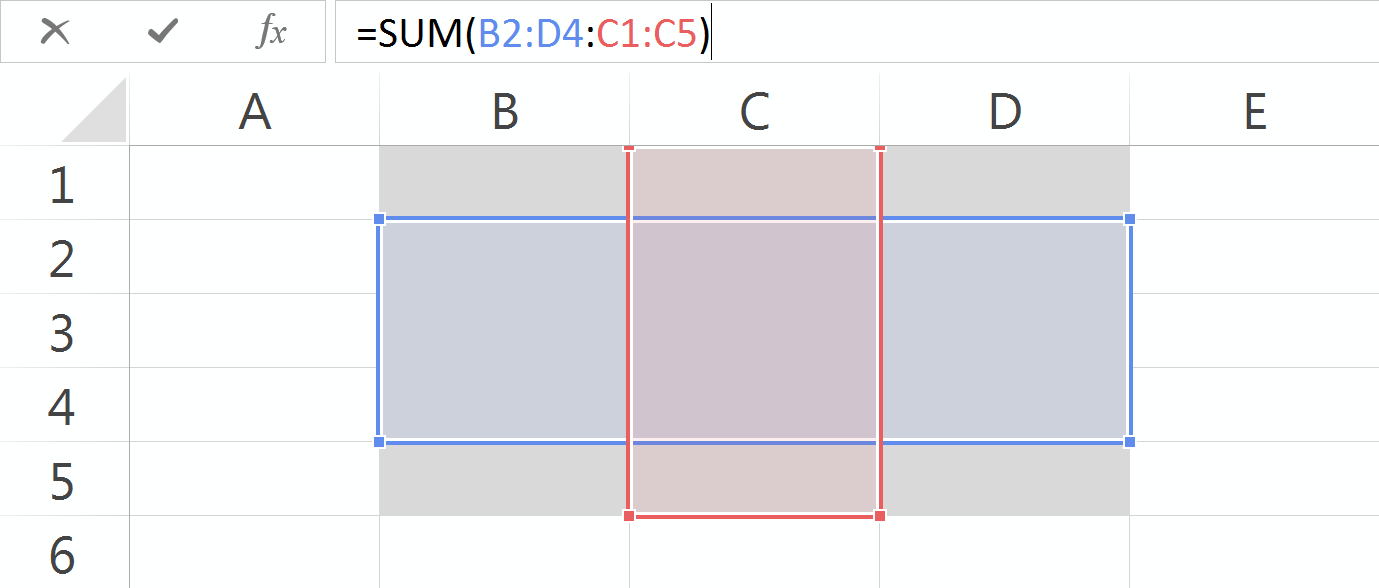
\includegraphics[width=1\textwidth]{img/complexRanges}
		\caption{A range with four limits \texttt{B2:D4:C1:C5}, equivalent to the area marked gray \texttt{B1:D5}}
		\label{fig:complexA}
	\end{subfigure}
	~ %add desired spacing between images, e. g. ~, \quad, \qquad, \hfill etc. 
	%(or a blank line to force the subfigure onto a new line)
	\begin{subfigure}[b]{0.47\textwidth}
		\centering
		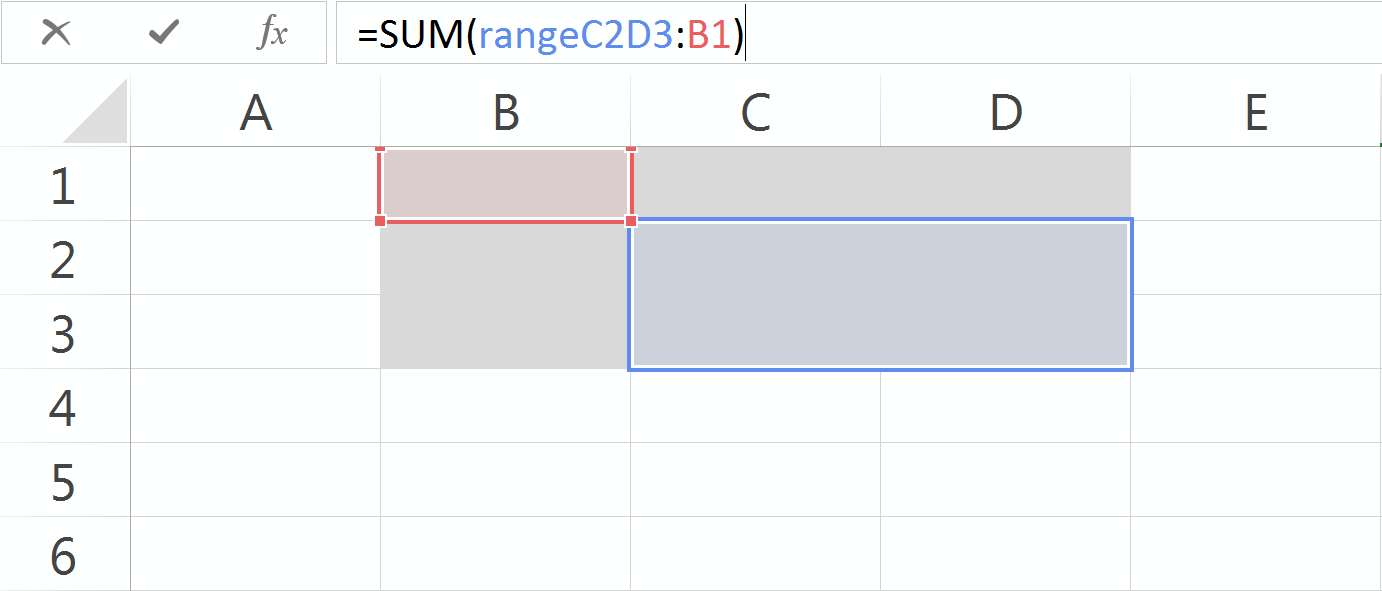
\includegraphics[width=1\textwidth]{img/complexNamedRanges}
		\caption{A range with a named range \texttt{rangeC2D3:B1}, equivalent to the area marked gray \texttt{A1:C3}}
		\label{fig:complexB}
	\end{subfigure}
	\caption{Examples of references to complex ranges}\label{Figure:ComplexRanges}
\end{figure}

By \textit{complex ranges} we mean \synt{Reference}s that include more than two or different types of \texttt{':'} separated \synt{ReferenceItem}s. An example is range \texttt{B2:D4:C1:C5}, illustrated in Figure \ref{fig:complexA}. The smelly aspect of complex ranges is their evaluation. Simple cell ranges are in the form \texttt{top-left:bottom-right}, including all cells in between the two limits. However, the limits in complex ranges are not the ones specified in the formula: they are calculated as the upper leftmost and lower rightmost cell in the square that includes all defined cells. For example, range \texttt{B2:D4:C1:C5} is equivalent to \texttt{B1:D5}. Understanding the limits of the range becomes even less intuitive when vertical or horizontal ranges or named ranges are used, like in Figure \ref{fig:complexB}. This syntax does not add to expressiveness of the grammar: each range is still calculated as the cells within a single square, but without clearly user-defined limits. Complex ranges are rare: 8,581 formulas	(0.04\%) include complex ranges in the Enron dataset, and they are all defined using three cell locations. 

The \textit{intersect operator} is included in this discussion because it is \texttt{\char32}, a single whitespace.
An advantage of this approach is that it enables more natural language definition of intersections, e.g. \texttt{=SUM((Total_Cost Jan):(Total_Cost Apr.))}.
However, we find this representation inconsistent to the grammar, because whitespace does not carry meaning in the rest of the language. Other spreadsheet systems do not use whitespace for this operator, either by using an alternative like LibreOffice which uses \texttt{!} or simply not supporting it. In the four datasets intersection operations are rare, as they are found in only 2,343 formulas (0.01\%).

\section{Discussion and Limitations}
\label{sec:discussion}
The currently defined formula grammar is able to parse 99,99\% of the 8,577,426 unique formulas in the four datasets. In this section, we discuss a variety of issues that affect its applicability and suitability.

\subsection{Dialects}

While other spreadsheet programs (e.g. Numbers, LibreOffice, Google Sheets) have generally adopted the Excel formula syntax, there are slight differences between programs and even Excel versions.
The grammar has been designed as a generically as possible and has been enriched to include all syntactical features found in the four datasets.
Both datasets, however, contain spreadsheets created in, or converted to, the Excel 2007 format.
This limits the grammar support for language elements that are spreadsheet system-dependent or even version-dependent.
The built-in functions list for example might change across versions, which would make the parser mistakenly recognize built-in functions as user-defined functions.
Another example is found in LibreOffice, which uses \texttt{\~} as the union operator instead of \texttt{,}.
The presented grammar will need to be modified to account for these differences before it can be used on other dialects.

Syntactical features have also been deprecated between Excel versions.
An example is regular expressions in formulas.
Excel allows defining formulas that include regular expressions, for example \texttt{=SUM('S*'!A1)} or \texttt{=SUM('Sheet?'!A1)}.
However, in Excel 2010 and up, regular expressions are instantly resolved---in the example, to  \texttt{=SUM(Sheet2:Sheet3!A1)}, summing up all A1 cells between Sheet2 and Sheet3, where the sheets are all sheets matching the regular expression, except the one that the formula is on.
This way, in Excel versions 2010 and up, saved spreadsheets never contain regular expressions.
\begin{figure}
	\centering
	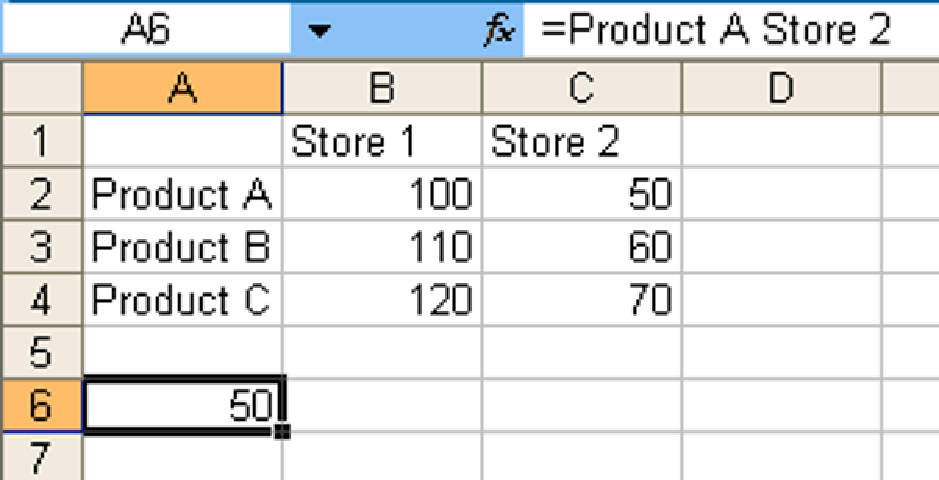
\includegraphics[width=0.4\textwidth]{img/labels}
	\caption{A natural language formula in Excel 2003}
	\label{fig:labels}
\end{figure}

The use of labels in formulas (referred to as natural language formulas) is another feature that was discontinued in Excel 2007.
Labels were the headings that were typed above columns and before rows, and they could be used in formulas instead of defined names or cell ranges.
Figure \ref{fig:labels} shows an example in Excel 2003, where formula \texttt{=Product A Store 2} returns the intersection between the cell range with heading \texttt{Product A} and the one with heading \texttt{Store 2}.
This feature is replaced in newer versions of Excel with the less error-prone named ranges feature.
When processing spreadsheets with newer versions of Excel, the references that include labels are automatically converted to cell-only references---in the example, the formula is converted to \texttt{=C2}.
The grammar does not support labels, and it would mistakenly parse them as named ranges.

\subsection{Internationalization}

Excel formulas differ depending on the language of the software. For example function arguments are separated by a semicolon instead of a comma in locales that use the comma as a decimal separator: the formula \texttt{=SUM(1.5,A1)} in the English version would be shown as \texttt{=SOM(1,5;A1)} in the Dutch version.
Our grammar supports only the English locale.
Grammars for other locales can be derived by replacing delimiters, error values and function names with their localized versions.

It is worth noting that Excel will always save formulas in either a locale-independent form (Excel 2003 and earlier format) or in its English version (Excel 2007 and later format). When interacting with Excel through its API two versions of the formula can be read or written: the English version and the version in the current locale.
This makes a grammar for the English version useful, since the parser can process all spreadsheets as long as their formulas are read using the always available English locale.

\subsection{Rejection of Invalid Formulas}

As stated in the design goals in Section \ref{sec:designgoals}, the goal of this grammar is to facilitate analysis of formulas, which means correctly parsing valid spreadsheet formulas.
Rejecting invalid formulas is not among the primary goals of this grammar, as the parser will normally not encounter invalid formulas in Excel files.
Furthermore, while there exist three big datasets of valid formulas, no such datasets of invalid formulas exist.
As such we expect that the presented grammar will parse formulas which are not valid.
Using this grammar to parse possibly-invalid formulas like user-input might thus require additional safeguards.

On one point we know the grammar to be too broad: Excel places several limitation on formulas like the number of arguments of a function (255), nested function calls (64), row number ($2^{20}$), column number ($2^{14}$) and total formula length ($2^{13}$), with lower numbers in older file formats.
Our grammar does not incorporate any of these limits.

\subsection{Parse Tree Correctness}

While we have empirically shown a high compatibility in terms of successful parse rate, we do not have as much evidence that the produced parse trees are correct as this is only tested by usage and unit tests in the reference implementation. We have manually sampled numerous parse trees and we have found them to be correct. We believe it is unlikely that a formula parsed with the presented grammar would be interpreted differently by Excel, but we do seek additional feedback on possible erroneous parse trees from the research community.

\section{Related Work}
\label{section:relatedWork}
Efforts to reverse-engineer language characteristics based on existing artifacts have been successful for other languages, including COBOL \cite{van1997obtaining} and C, C++, C\# and Java \cite{zaytsev2010recovery}.

Most related to our research on the spreadsheet formula language is the work of Badame and Dig~\cite{badame2012refactoring} who, as part of their proposed spreadsheet refactoring approach, presented a grammar for spreadsheet formulas. However, they do not evaluate their grammar, and upon inspection one can see that key ingredients are missing: e.g. external references, intersections, unions, named ranges and operator precedence. An extension of the same grammar was used to refactor formulas by Hermans and Dig \cite{hermans2014bumblebee}.

There is a large body of related work that relies on parsing spreadsheet formulas to analyze spreadsheets. This includes our own work in which we have created an algorithm to visualize spreadsheets as dataflow diagrams \cite{DBLP:conf/icse/HermansPD11}, and subsequently on detecting smells in spreadsheets \cite{DBLP:conf/icse/HermansPD12,DBLP:conf/icsm/Hermans212}. Related approaches exist, for example the work of Cunha that have worked on code smells~\cite{iccsa12} and smell-based fault localization~\cite{conf/icsme/CunhaFMPS14}. These papers also analyze spreadsheet formulas but do not detail which grammar or analysis method they use.

\section{Conclusion}
\label{section:conclusion}
In this paper we (1) present a grammar for spreadsheet formulas, (2) evaluate it against over eight million unique formulas, successfully parsing 99.99\%, and (3) use it to analyze the formulas in the dataset, measure the frequency of their characteristics and find uncommon grammatical cases.

The grammar is compact and produces processable parse trees, suited for further manipulation and analysis. We believe that the grammar is reliable and concise enough to facilitate further research on spreadsheet formula codebases. It has already been applied in other works for analyzing formula characteristics, calculation chains and code smells and for applying formula transformations. The XLParser\footnote{\url{https://github.com/PerfectXL/XLParser}} is published as open-source software and an online demo is also available.\footnote{\url{http://xlparser.perfectxl.nl/demo}}

A point of improvement for the grammar is that its exact compatibility with the official Excel grammar is unknown.
A comparison to the official specification could lead to either improving compatibility, or extending the number of known limitations.
In general, the problem of determining whether two context-free grammars are equivalent is undecidable, but in practice several techniques have been successfully used for this purpose \cite{lammel2009introduction,fischer2012comparison}.

\bibliographystyle{wileyj}
\bibliography{XLGrammarRefs}

\end{document}
